
%% bare_conf.tex
%% V1.3
%% 2007/01/11
%% by Michael Shell
%% See:
%% http://www.michaelshell.org/
%% for current contact information.
%%
%% This is a skeleton file demonstrating the use of IEEEtran.cls
%% (requires IEEEtran.cls version 1.7 or later) with an IEEE conference paper.
%%
%% Support sites:
%% http://www.michaelshell.org/tex/ieeetran/
%% http://www.ctan.org/tex-archive/macros/latex/contrib/IEEEtran/
%% and
%% http://www.ieee.org/

%%*************************************************************************
%% Legal Notice:
%% This code is offered as-is without any warranty either expressed or
%% implied; without even the implied warranty of MERCHANTABILITY or
%% FITNESS FOR A PARTICULAR PURPOSE! 
%% User assumes all risk.
%% In no event shall IEEE or any contributor to this code be liable for
%% any damages or losses, including, but not limited to, incidental,
%% consequential, or any other damages, resulting from the use or misuse
%% of any information contained here.
%%
%% All comments are the opinions of their respective authors and are not
%% necessarily endorsed by the IEEE.
%%
%% This work is distributed under the LaTeX Project Public License (LPPL)
%% ( http://www.latex-project.org/ ) version 1.3, and may be freely used,
%% distributed and modified. A copy of the LPPL, version 1.3, is included
%% in the base LaTeX documentation of all distributions of LaTeX released
%% 2003/12/01 or later.
%% Retain all contribution notices and credits.
%% ** Modified files should be clearly indicated as such, including  **
%% ** renaming them and changing author support contact information. **
%%
%% File list of work: IEEEtran.cls, IEEEtran_HOWTO.pdf, bare_adv.tex,
%%                    bare_conf.tex, bare_jrnl.tex, bare_jrnl_compsoc.tex
%%*************************************************************************

% *** Authors should verify (and, if needed, correct) their LaTeX system  ***
% *** with the testflow diagnostic prior to trusting their LaTeX platform ***
% *** with production work. IEEE's font choices can trigger bugs that do  ***
% *** not appear when using other class files.                            ***
% The testflow support page is at:
% http://www.michaelshell.org/tex/testflow/



% Note that the a4paper option is mainly intended so that authors in
% countries using A4 can easily print to A4 and see how their papers will
% look in print - the typesetting of the document will not typically be
% affected with changes in paper size (but the bottom and side margins will).
% Use the testflow package mentioned above to verify correct handling of
% both paper sizes by the user's LaTeX system.
%
% Also note that the "draftcls" or "draftclsnofoot", not "draft", option
% should be used if it is desired that the figures are to be displayed in
% draft mode.
%
\documentclass[journal,12pt]{IEEEtran}
% Add the compsoc option for Computer Society conferences.
%
% If IEEEtran.cls has not been installed into the LaTeX system files,
% manually specify the path to it like:
% \documentclass[conference]{../sty/IEEEtran}





% Some very useful LaTeX packages include:
% (uncomment the ones you want to load)


% *** MISC UTILITY PACKAGES ***
%
%\usepackage{ifpdf}
% Heiko Oberdiek's ifpdf.sty is very useful if you need conditional
% compilation based on whether the output is pdf or dvi.
% usage:
% \ifpdf
%   % pdf code
% \else
%   % dvi code
% \fi
% The latest version of ifpdf.sty can be obtained from:
% http://www.ctan.org/tex-archive/macros/latex/contrib/oberdiek/
% Also, note that IEEEtran.cls V1.7 and later provides a builtin
% \ifCLASSINFOpdf conditional that works the same way.
% When switching from latex to pdflatex and vice-versa, the compiler may
% have to be run twice to clear warning/error messages.






% *** CITATION PACKAGES ***
%
\usepackage{cite}
% cite.sty was written by Donald Arseneau
% V1.6 and later of IEEEtran pre-defines the format of the cite.sty package
% \cite{} output to follow that of IEEE. Loading the cite package will
% result in citation numbers being automatically sorted and properly
% "compressed/ranged". e.g., [1], [9], [2], [7], [5], [6] without using
% cite.sty will become [1], [2], [5]--[7], [9] using cite.sty. cite.sty's
% \cite will automatically add leading space, if needed. Use cite.sty's
% noadjust option (cite.sty V3.8 and later) if you want to turn this off.
% cite.sty is already installed on most LaTeX systems. Be sure and use
% version 4.0 (2003-05-27) and later if using hyperref.sty. cite.sty does
% not currently provide for hyperlinked citations.
% The latest version can be obtained at:
% http://www.ctan.org/tex-archive/macros/latex/contrib/cite/
% The documentation is contained in the cite.sty file itself.






% *** GRAPHICS RELATED PACKAGES ***
%
\ifCLASSINFOpdf
  \usepackage[pdftex]{graphicx}
  % declare the path(s) where your graphic files are
  \graphicspath{{./images/}}
  % and their extensions so you won't have to specify these with
  % every instance of \includegraphics
  % \DeclareGraphicsExtensions{.pdf,.jpeg,.png}
\else
  % or other class option (dvipsone, dvipdf, if not using dvips). graphicx
  % will default to the driver specified in the system graphics.cfg if no
  % driver is specified.
  % \usepackage[dvips]{graphicx}
  % declare the path(s) where your graphic files are
  % \graphicspath{{../eps/}}
  % and their extensions so you won't have to specify these with
  % every instance of \includegraphics
  % \DeclareGraphicsExtensions{.eps}
\fi
% graphicx was written by David Carlisle and Sebastian Rahtz. It is
% required if you want graphics, photos, etc. graphicx.sty is already
% installed on most LaTeX systems. The latest version and documentation can
% be obtained at: 
% http://www.ctan.org/tex-archive/macros/latex/required/graphics/
% Another good source of documentation is "Using Imported Graphics in
% LaTeX2e" by Keith Reckdahl which can be found as epslatex.ps or
% epslatex.pdf at: http://www.ctan.org/tex-archive/info/
%
% latex, and pdflatex in dvi mode, support graphics in encapsulated
% postscript (.eps) format. pdflatex in pdf mode supports graphics
% in .pdf, .jpeg, .png and .mps (metapost) formats. Users should ensure
% that all non-photo figures use a vector format (.eps, .pdf, .mps) and
% not a bitmapped formats (.jpeg, .png). IEEE frowns on bitmapped formats
% which can result in "jaggedy"/blurry rendering of lines and letters as
% well as large increases in file sizes.
%
% You can find documentation about the pdfTeX application at:
% http://www.tug.org/applications/pdftex





% *** MATH PACKAGES ***
%
\usepackage[cmex10]{amsmath}
% A popular package from the American Mathematical Society that provides
% many useful and powerful commands for dealing with mathematics. If using
% it, be sure to load this package with the cmex10 option to ensure that
% only type 1 fonts will utilized at all point sizes. Without this option,
% it is possible that some math symbols, particularly those within
% footnotes, will be rendered in bitmap form which will result in a
% document that can not be IEEE Xplore compliant!
%
% Also, note that the amsmath package sets \interdisplaylinepenalty to 10000
% thus preventing page breaks from occurring within multiline equations. Use:
%\interdisplaylinepenalty=2500
% after loading amsmath to restore such page breaks as IEEEtran.cls normally
% does. amsmath.sty is already installed on most LaTeX systems. The latest
% version and documentation can be obtained at:
% http://www.ctan.org/tex-archive/macros/latex/required/amslatex/math/





% *** SPECIALIZED LIST PACKAGES ***
%
%\usepackage{algorithmic}
% algorithmic.sty was written by Peter Williams and Rogerio Brito.
% This package provides an algorithmic environment fo describing algorithms.
% You can use the algorithmic environment in-text or within a figure
% environment to provide for a floating algorithm. Do NOT use the algorithm
% floating environment provided by algorithm.sty (by the same authors) or
% algorithm2e.sty (by Christophe Fiorio) as IEEE does not use dedicated
% algorithm float types and packages that provide these will not provide
% correct IEEE style captions. The latest version and documentation of
% algorithmic.sty can be obtained at:
% http://www.ctan.org/tex-archive/macros/latex/contrib/algorithms/
% There is also a support site at:
% http://algorithms.berlios.de/index.html
% Also of interest may be the (relatively newer and more customizable)
% algorithmicx.sty package by Szasz Janos:
% http://www.ctan.org/tex-archive/macros/latex/contrib/algorithmicx/




% *** ALIGNMENT PACKAGES ***
%
%\usepackage{array}
% Frank Mittelbach's and David Carlisle's array.sty patches and improves
% the standard LaTeX2e array and tabular environments to provide better
% appearance and additional user controls. As the default LaTeX2e table
% generation code is lacking to the point of almost being broken with
% respect to the quality of the end results, all users are strongly
% advised to use an enhanced (at the very least that provided by array.sty)
% set of table tools. array.sty is already installed on most systems. The
% latest version and documentation can be obtained at:
% http://www.ctan.org/tex-archive/macros/latex/required/tools/


%\usepackage{mdwmath}
%\usepackage{mdwtab}
% Also highly recommended is Mark Wooding's extremely powerful MDW tools,
% especially mdwmath.sty and mdwtab.sty which are used to format equations
% and tables, respectively. The MDWtools set is already installed on most
% LaTeX systems. The lastest version and documentation is available at:
% http://www.ctan.org/tex-archive/macros/latex/contrib/mdwtools/


% IEEEtran contains the IEEEeqnarray family of commands that can be used to
% generate multiline equations as well as matrices, tables, etc., of high
% quality.


%\usepackage{eqparbox}
% Also of notable interest is Scott Pakin's eqparbox package for creating
% (automatically sized) equal width boxes - aka "natural width parboxes".
% Available at:
% http://www.ctan.org/tex-archive/macros/latex/contrib/eqparbox/





% *** SUBFIGURE PACKAGES ***
\usepackage[tight,footnotesize]{subfigure}
% subfigure.sty was written by Steven Douglas Cochran. This package makes it
% easy to put subfigures in your figures. e.g., "Figure 1a and 1b". For IEEE
% work, it is a good idea to load it with the tight package option to reduce
% the amount of white space around the subfigures. subfigure.sty is already
% installed on most LaTeX systems. The latest version and documentation can
% be obtained at:
% http://www.ctan.org/tex-archive/obsolete/macros/latex/contrib/subfigure/
% subfigure.sty has been superceeded by subfig.sty.



%\usepackage[caption=false]{caption}
%\usepackage[font=footnotesize]{subfig}
% subfig.sty, also written by Steven Douglas Cochran, is the modern
% replacement for subfigure.sty. However, subfig.sty requires and
% automatically loads Axel Sommerfeldt's caption.sty which will override
% IEEEtran.cls handling of captions and this will result in nonIEEE style
% figure/table captions. To prevent this problem, be sure and preload
% caption.sty with its "caption=false" package option. This is will preserve
% IEEEtran.cls handing of captions. Version 1.3 (2005/06/28) and later 
% (recommended due to many improvements over 1.2) of subfig.sty supports
% the caption=false option directly:
%\usepackage[caption=false,font=footnotesize]{subfig}
%
% The latest version and documentation can be obtained at:
% http://www.ctan.org/tex-archive/macros/latex/contrib/subfig/
% The latest version and documentation of caption.sty can be obtained at:
% http://www.ctan.org/tex-archive/macros/latex/contrib/caption/




% *** FLOAT PACKAGES ***
%
%\usepackage{fixltx2e}
% fixltx2e, the successor to the earlier fix2col.sty, was written by
% Frank Mittelbach and David Carlisle. This package corrects a few problems
% in the LaTeX2e kernel, the most notable of which is that in current
% LaTeX2e releases, the ordering of single and double column floats is not
% guaranteed to be preserved. Thus, an unpatched LaTeX2e can allow a
% single column figure to be placed prior to an earlier double column
% figure. The latest version and documentation can be found at:
% http://www.ctan.org/tex-archive/macros/latex/base/



%\usepackage{stfloats}
% stfloats.sty was written by Sigitas Tolusis. This package gives LaTeX2e
% the ability to do double column floats at the bottom of the page as well
% as the top. (e.g., "\begin{figure*}[!b]" is not normally possible in
% LaTeX2e). It also provides a command:
%\fnbelowfloat
% to enable the placement of footnotes below bottom floats (the standard
% LaTeX2e kernel puts them above bottom floats). This is an invasive package
% which rewrites many portions of the LaTeX2e float routines. It may not work
% with other packages that modify the LaTeX2e float routines. The latest
% version and documentation can be obtained at:
% http://www.ctan.org/tex-archive/macros/latex/contrib/sttools/
% Documentation is contained in the stfloats.sty comments as well as in the
% presfull.pdf file. Do not use the stfloats baselinefloat ability as IEEE
% does not allow \baselineskip to stretch. Authors submitting work to the
% IEEE should note that IEEE rarely uses double column equations and
% that authors should try to avoid such use. Do not be tempted to use the
% cuted.sty or midfloat.sty packages (also by Sigitas Tolusis) as IEEE does
% not format its papers in such ways.





% *** PDF, URL AND HYPERLINK PACKAGES ***
%
%\usepackage{url}
% url.sty was written by Donald Arseneau. It provides better support for
% handling and breaking URLs. url.sty is already installed on most LaTeX
% systems. The latest version can be obtained at:
% http://www.ctan.org/tex-archive/macros/latex/contrib/misc/
% Read the url.sty source comments for usage information. Basically,
% \url{my_url_here}.





% *** Do not adjust lengths that control margins, column widths, etc. ***
% *** Do not use packages that alter fonts (such as pslatex).         ***
% There should be no need to do such things with IEEEtran.cls V1.6 and later.
% (Unless specifically asked to do so by the journal or conference you plan
% to submit to, of course. )


% correct bad hyphenation here
\hyphenation{op-tical net-works semi-conduc-tor}
\usepackage{listings}
\usepackage{amsfonts}
\graphicspath{{./img/}}
\begin{document}
%
% paper title
% can use linebreaks \\ within to get better formatting as desired



% author names and affiliations
% use a multiple column layout for up to three different
% affiliations
\title{\vspace{-0.05\textheight}Human Computer Interaction 2011\\\large{Assignment 1: Image Labelling Application}}

\author{
\IEEEauthorblockN{Behzad Tabibian and William Ogilvie}\\
\IEEEauthorblockA{School of Informatics\\University of Edinburgh\\}
}


% conference papers do not typically use \thanks and this command
% is locked out in conference mode. If really needed, such as for
% the acknowledgment of grants, issue a \IEEEoverridecommandlockouts
% after \documentclass

% for over three affiliations, or if they all won't fit within the width
% of the page, use this alternative format:
% 
%\author{\IEEEauthorblockN{Michael Shell\IEEEauthorrefmark{1},
%Homer Simpson\IEEEauthorrefmark{2},
%James Kirk\IEEEauthorrefmark{3}, 
%Montgomery Scott\IEEEauthorrefmark{3} and
%Eldon Tyrell\IEEEauthorrefmark{4}}
%\IEEEauthorblockA{\IEEEauthorrefmark{1}School of Electrical and Computer Engineering\\
%Georgia Institute of Technology,
%Atlanta, Georgia 30332--0250\\ Email: see http://www.michaelshell.org/contact.html}
%\IEEEauthorblockA{\IEEEauthorrefmark{2}Twentieth Century Fox, Springfield, USA\\
%Email: homer@thesimpsons.com}
%\IEEEauthorblockA{\IEEEauthorrefmark{3}Starfleet Academy, San Francisco, California 96678-2391\\
%Telephone: (800) 555--1212, Fax: (888) 555--1212}
%\IEEEauthorblockA{\IEEEauthorrefmark{4}Tyrell Inc., 123 Replicant Street, Los Angeles, California 90210--4321}}




% use for special paper notices
%\IEEEspecialpapernotice{(Invited Paper)}




% make the title area
\maketitle


%\begin{abstract}
%\boldmath
%The abstract goes here.
%\end{abstract}
% IEEEtran.cls defaults to using nonbold math in the Abstract.
% This preserves the distinction between vectors and scalars. However,
% if the conference you are submitting to favors bold math in the abstract,
% then you can use LaTeX's standard command \boldmath at the very start
% of the abstract to achieve this. Many IEEE journals/conferences frown on
% math in the abstract anyway.

% no keywords




% For peer review papers, you can put extra information on the cover
% page as needed:
% \ifCLASSOPTIONpeerreview
% \begin{center} \bfseries EDICS Category: 3-BBND \end{center}
% \fi
%
% For peerreview papers, this IEEEtran command inserts a page break and
% creates the second title. It will be ignored for other modes.
\IEEEpeerreviewmaketitle
	


\section{Introduction}
Here goes the introduction
\section{Image Annotation}
Image annotation in this program uses a set of vertices which form a polygon to distinguish the object from the rest of the image. User, once clicked on "Add" button, can select any where on the screen and start drawing the polygon. When finished, right click on the picture or click on "Add" button again finishes drawing.Then, A window will pop up and asks for a name for annotated part of the picture, This window is modal window provided by the framework and is an standard way of getting small inputs. Names appear as a tool-tip of each annotation.

There are several remarks about this feature. One problem that we had to deal with was that users may not select the vertices of the polygon in order. This situations is not supported by the underlying framework and produces undefined shapes. Our solution to this problem was to colour the surface of the polygon as user adds vertices. This results to an intuition for the user which prevents him to add a vertex Between to vertex of the polygon.

We also dropped editing position of each vertex of a polygon. Therefore, once user adds an annotation he can not change it unless annotation is deleted and redrawn. This design decision was based on time constraints that we had and other features that we wanted to implement. Also , in practice, annotations are usually small and therefore user prefers to redraw the object rather than changing and/or adding extra vertices to an already drawn polygon.
\section{Zooming}
The zoom feature for the image annotation project was based upon those found in Internet browser software such as FireFox and Safari, and it comprises three main functions: zoom in, zoom out, and reset zoom.  Since browsers are arguably the most frequently used software on a computer it seemed natural to follow their implementations of this feature.  This included using the same shortcut keys as those found in browser software.  As a partially sighted person William naturally finds himself hitting these key combinations first whenever he want to zoom in or out of an object on the screen, and anecdotal evidence suggests to him that this has become the de facto standard; whenever an application doesn’t follow this convention he finds it initially confusing and then increasingly irritating as he has to  hunt around the menu structure to see if this feature is even implemented.  We consider this very poor design practice and this is why we chose to implement the zoom feature in this way.

In terms of criticisms, the zoom feature was designed to scale the entire image up and down at the user’s discretion.  This is contrary to some other image editing software packages which chose to implement this feature in a different way.  The alternative method is to have a single function that, depending upon where you click, will zoom and center on a particular location on the left-click of a mouse, and zoom out upon a right-click.  This can be useful when the user wishes to edit an image in fine detail; however, the primary use case of this product seems to suggest that annotations will not require fine detail creation and hence this is why it was implemented in this way.  Still, this is a design decision and should be considered a legitimate concern.  If this were a commercial product usability testing would be useful to bore out which method is more conducive to the programs users.
\section{Fast Browsing}
The fast browsing capabilities of this product consist of two docks.  One holds the hierarchical file structure of the system and the other is a thumbnail viewer.  The thumbnail viewer dock is directly linked in functionality to the file viewer dock in that it displays the images found in the deepest expanded folder in the file system tree.  Both docks can be used to open an image file by double clicking on the respective icon or image.  This allows a user to open image files more quickly without the use of the open dialog box in the file menu, and hence makes it easier to annotate multiple images at once, or indeed browse to find the correct image the user was looking for if they are unsure of the file name.

These docks have been deliberately placed at the left side of the application by default, although they are able to be individually dragged to the right side if the user so chooses or simply allowed to float at a desired location.  The reason these features were placed in this way is based upon the observation that navigation controls typically reside to left of the screen.  From the Windows Explorer application in Microsoft Windows 95, to the Facebook website, to the integrated development environment used to construct this product, navigation controls more often than not are placed to the left hand side of the screen.  This has become the unwritten convention and would be foolish to ignore without good cause.

In evaluating the implementation of the fast browsing features there are two main negative comments one could make.  The first relates to the fact that an action on one dock, expanding or collapsing a folder, has a direct impact upon another dock, the thumbnails change.  Due to that connection a person may argue that these controls should be present on the same dock to avoid confusion.  By having these two controls on top of each other in a single dock it may be true to say that it would be clearer that they inter-operate with each other; however, we would argue that this ignores the cases where a user wishes to only navigate through the folder structure and doesn’t want a thumbnail viewer shown on their workspace - or vice-versa.  The other criticism is that there is no mechanism, through a shortcut key or otherwise, for a user to skip from one image to the next within a single folder when batch annotating multiple images without using the mouse.  In defense of this fact we would argue that since the act of annotating images requires heavy use of the mouse, providing keyboard navigation shortcuts would not make batch image annotation any faster.

\section{Save\slash Load}
A key feature of this package is the ability to save annotations made to an image and load them automatically when viewing it later. To do this the program saves the locations of every vertex, along with the name of each annotation, within an XML file.  This XML file is stored within the same directory in which the original image resides and the data loaded back when the user reopens that image file.

The XML format was chosen for saving the annotations for two reasons. First, we needed a standard method of storing the meta-data of the image and the widely adopted format for this is XML: probably the main reason for this is that XML can easily inter-operate with multiple applications.  The other reason XML was chosen was that we wanted to make the stored information human-readable, so that when the file is opened in a text editor the user can read and edit the annotations themselves if they so desire.

The image annotation program loads the meta-data of every image automatically, if the appropriate XML file exists in the same directory under the name of that image. This scheme of storing information was chosen to prevent making databases of labels. This has some advantages and disadvantage. One advantage is that there is no need to fetch and alter the labels of a specific image; depending upon the schema of a database, this can be computationally expensive if large numbers of images are considered. Also this method keeps the security of the meta-data at the same level as the images themselves, so when a user does not have access to an image they will not be able to read the annotations either.  By extension, if the user has read-only access they will only be able to read the annotations too. A drawback of this method of storing information is that it would not be easy to implement other features such as search; however, since the use case of this package does not cover it this method was deemed most appropriate.

Many software applications also check for user changes to current file each time a new image is being opened or application is going to close. In our implementation of this feature each time user adds or removes a label or when an annotation is moved, program stores these changes and when a new image is to be opened or when application is closing, asks user whether it should save them or not 

An example file produced by the application can be found in listing \ref{lst:svd} below.    

\begin{center}
\lstset{language=XML, basicstyle=\footnotesize\ttfamily, caption=XML file used to store image labels,frame=single,captionpos=b,label=lst:svd}
\lstinputlisting{svd.txt}
\end{center}

\section{Menu and Shortcuts}
The layout of the standard menu structure has been fixed for a great many years, and in creating this application we have tried to stick to these conventions.  We have implemented a "File" menu containing "Open", "Save", and "Exit" commands; we created an "Edit"  menu with add and delete annotation commands; and we have a "View" menu where the user can control which docks they wish to see, and at which zoom level the image viewer should be set.  There isn’t a great deal that can be said for this particular layout, nearly every application has had these menu items in this precise order for at least the past fifteen years, except to mention that in terms of human computer interactions, and where a user expects commands to be located, a GUI designer should ignore this convention at their peril.

We have tried to stick to convention again when choosing the shortcut keys for the main menu items, particularly when it came to the file system commands.  The items file, open, save, and exit usually the have same keyboard bindings in all applications and so we have not altered this since we do not wish to confuse the user.  As previously mentioned, the bindings for the zoom feature have been taken from those present in most Internet browsers.  In terms of software, these applications are amongst the most used on a computer today: thus following their standards seemed wise.  Unfortunately when it came to the annotation commands there were no such well-known templates to follow, and so it was down to common sense to provide the answer.  Add annotation begins with the letter a and so that was chosen to represent that action.  Following the same logic the letter d might have been chosen for the delete action, except that the QWERTY keyboard layout already has two keys dedicated to this task - delete and backspace.  In the end, backspace was chosen since it is more familiar to unsophisticated users and hence they are more likely to associate it with a delete action.

We also included a status bar at the bottom of the application.  This displays context-sensitive text depending upon where the mouse is hovering.  This is common in many applications and we hope that this will aid users in the use of this package.

\section{Action Suggestion}
Action suggestion is a special feature of this software package. The goal is to demonstrate how probabilistic Machine Learning can be used in the User Interface stack of a variety of applications. To demonstrate this, we modelled user actions with elements of probability distributions to infer the next possible action of the user; the model is then updated according to the past experiences that are observed. A suggested action is shown in a separate dock widget on the left side of the screen, and as discussed earlier the user can move them to another position on the screen if desired. Mathematical derivation of the model is not described here but can be found in the appendix.

To build this model we made some assumptions about user actions:
\begin{itemize}
\item Next action of the user only depends on its previous action.
\item Number of possible actions are limited and discrete.
\end{itemize}
These assumptions are made to make the model simpler and possible to implement and test within the time limits of this assignment. We assume the user has four actions: {\textit{Add}, \textit{Delete}, \textit{Open}, and \textit{Save}}. Also the program is preloaded with some prior information about user behaviour after each action. Prior information can be found in table \ref{tab:priors}. This table can be interpreted as the number of times users have chosen a specific action after the action specified in the first column is observed.
\begin{table}[t]
\centering
\begin{tabular}{|c|c|c|c|c|}
\hline \rule[-1ex]{0pt}{3.5ex}  & OPEN & SAVE & EDIT & ADD \\ 
\hline \rule[-1ex]{0pt}{3.5ex} OPEN & 1 & 1 & 3 & 5 \\ 
\hline \rule[-1ex]{0pt}{3.5ex} SAVE & 4 & 1 & 2 & 3 \\ 
\hline \rule[-1ex]{0pt}{3.5ex} EDIT & 0 & 3 & 4 & 3 \\ 
\hline \rule[-1ex]{0pt}{3.5ex} ADD & 1 & 3 & 3 & 3 \\ 
\hline 
\end{tabular}
\caption{priors used for each action}
\label{tab:priors}
\end{table}
Once the program is loaded and the user starts loading images and annotating them their actions will be learnt and used for the next suggestions. For example, if a user opens an image after a new annotation, probability of suggesting that action is increased in later itterations.

Even though no empirical experiment was conducted certain patterns can be observed from a users behaviour which this model can capture. An example of such patterns can be seen when a user saves a file and then opens an image, or when a new image is loaded.  The user then usually starts adding labels to the loaded image. Both of these patterns are produced by the implemented inference system and suggestions are made according to action of the user.
This feature, however, cannot capture all possible patterns, for example it may not be able to suggest reasonable actions after the user has added a new label. This pattern may be modelled if the number of consecutive additions are taken into account. This and many other examples require more sophisticated mathematical models which are not present in this project.

\section{Conclusion}

In conclusion, the participant in our tests seemed happy with the program after learning how to use it.  However, looking at the interface implementation from a more professional point of view it is clear that some mistakes have been made.  For one thing, there should not be a 50 second plus learning curve on opening an image file.  This is one of the simplest operations a desktop application can make, and this confusion was entirely avoidable had the designers taken the time to implement the standard main menu, File sub-menu pattern found in so many applications.

Having ignored that convention, the programmers placed a vital user interface element at the far right of the window. It is well known in design, and has be born out by research carried out into eye movement tracking, that a person concentrates their gaze to the top and left of an application.  By placing the list of annotations on the far right they should have considered that it may be more difficult for a user to spot, and consequently re-thought that placement.  

Finally, it is typical in every day computer use that clicking on a UI component will either highlight or select it.  By separating the place where you select an annotation from the place where it is drawn you are disregarding this paradigm, and ultimately this may lead to the confusion of users.

Design deficiencies are clearly demonstrated in Figure \ref{fig:ave_rate} when the time to complete a task for the first time is plotted against user rating of how easy the task was.

\begin{figure}[t]
\centering
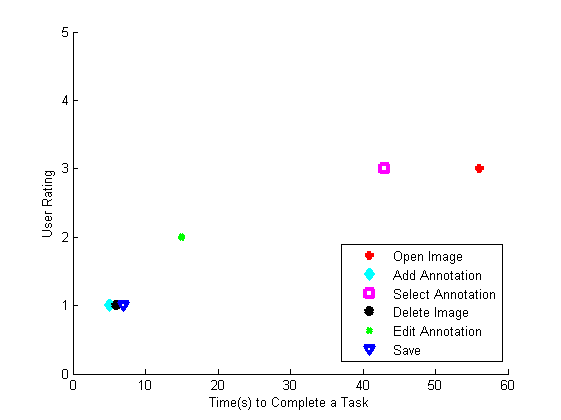
\includegraphics[width=8cm]{average_rating.png}
\caption{time takes for completing a task for the first time plotted against user rating of how easy it was to accomplish the task, lower number indicates task was easier. }
\label{fig:ave_rate}
\end{figure}

Since the application has fairly simple use cases it does get away with having a bit of a quirky layout, at least as far as our test subject was concerned.  However, in terms of following HCI principles, this application breaches a few too many and so we feel it would be better to redo the design in a more conventional manner so that users may be less confused while using it.

\renewcommand{\appendixname}{Appendix: Derivation of Bayesian Inference Engine }
\appendix
\section{Mathematical Derivation of Bayesian Inference Engine}
Every possible action of the user can be shown as a vector: $X_{act}=(open, save, edit, add)^T$ in which  $act \in {open, save, edit, add}$. Every action can be modelled as a \textit{Multinomial Distribution}:

\[
Mult(m_1,m_2,...,m_K|\mu,N)={N \choose m_1 m_2 ... m_K}\prod_{k=1}^K \mu_{k}^{x_k}
\]

where $\mu=(\mu_1,\mu_2,...,\mu_K)^T$. Finding the maximum likelihood solution for parameter $\mu$ will give us:

\[
\mu_k^{ML}={m_k \over N} 
\]

We use this result to approximate the best probability for the next action. It is natural to think about this result as averaging over the observations.
To take one step further and introduce priors to the distribution we use \textit{Dirichlet distribution} which is the conjugate prior of the multinomial distribution.
\[
Dir(\mu|\alpha)={\Gamma(\alpha_0) \over \Gamma(\alpha_1)...\Gamma(\alpha_K)}\prod_{k=1}^K \mu_{k}^{\alpha_k -1}
\]
Conjugate priors have certain characteristics which makes it easy to compute the posterior of the distribution that is constructed by multiplying the likelihood function by the prior.  
\[
p(D|\mu)=\prod_{k=1}^K {\mu_{k}^{m_k}}\]

\[p(\mu| D,\alpha) \propto p(D|\mu)  p(\mu|\alpha)\]

\[p(\mu|D, \alpha)={\Gamma(\alpha_0+N) \over {\Gamma(\alpha_1+m_1)...\Gamma(\alpha_K+m_K)}}\prod_{k=1}^K \mu_{k}^{\alpha_k+m_k-1}\]

Marginalizing over $\mu$ we get 

\[p(x=add|D)=\int_0^1 p(x=add|\mu)p(\mu|D) \mathrm{d}\mu\]
\[p(x=add|D)=\int_0^1 \mu p(\mu|D)\mathrm{d}\mu = \mathbb{E}[\mu|D]\]

The value of the last line is equal to

\[\mathbb{E}[\mu|D]={m_k+\alpha_k \over {N+\alpha_0}} \]

The result, just like earlier, can be interpreted as considering priors as imaginary observations.

After calculating the $\mu$ of every action the suggestion is produced by using the Inverse Transform method and a uniform distribution.

In conclusion, the resulting model even though simple is tractable and produces expected results which are fairly robust.

For further information the reader is referred to \cite{Bishop2007}. 



\bibliographystyle{IEEEtran}
\bibliography{bibliography}


% An example of a floating figure using the graphicx package.
% Note that \label must occur AFTER (or within) \caption.
% For figures, \caption should occur after the \includegraphics.
% Note that IEEEtran v1.7 and later has special internal code that
% is designed to preserve the operation of \label within \caption
% even when the captionsoff option is in effect. However, because
% of issues like this, it may be the safest practice to put all your
% \label just after \caption rather than within \caption{}.
%
% Reminder: the "draftcls" or "draftclsnofoot", not "draft", class
% option should be used if it is desired that the figures are to be
% displayed while in draft mode.
%
%\begin{figure}[!t]
%\centering
%\includegraphics[width=2.5in]{myfigure}
% where an .eps filename suffix will be assumed under latex, 
% and a .pdf suffix will be assumed for pdflatex; or what has been declared
% via \DeclareGraphicsExtensions.
%\caption{Simulation Results}
%\label{fig_sim}
%\end{figure}

% Note that IEEE typically puts floats only at the top, even when this
% results in a large percentage of a column being occupied by floats.


% An example of a double column floating figure using two subfigures.
% (The subfig.sty package must be loaded for this to work.)
% The subfigure \label commands are set within each subfloat command, the
% \label for the overall figure must come after \caption.
% \hfil must be used as a separator to get equal spacing.
% The subfigure.sty package works much the same way, except \subfigure is
% used instead of \subfloat.
%
%\begin{figure*}[!t]
%\centerline{\subfloat[Case I]\includegraphics[width=2.5in]{subfigcase1}%
%\label{fig_first_case}}
%\hfil
%\subfloat[Case II]{\includegraphics[width=2.5in]{subfigcase2}%
%\label{fig_second_case}}}
%\caption{Simulation results}
%\label{fig_sim}
%\end{figure*}
%
% Note that often IEEE papers with subfigures do not employ subfigure
% captions (using the optional argument to \subfloat), but instead will
% reference/describe all of them (a), (b), etc., within the main caption.


% An example of a floating table. Note that, for IEEE style tables, the 
% \caption command should come BEFORE the table. Table text will default to
% \footnotesize as IEEE normally uses this smaller font for tables.
% The \label must come after \caption as always.
%
%\begin{table}[!t]
%% increase table row spacing, adjust to taste
%\renewcommand{\arraystretch}{1.3}
% if using array.sty, it might be a good idea to tweak the value of
% \extrarowheight as needed to properly center the text within the cells
%\caption{An Example of a Table}
%\label{table_example}
%\centering
%% Some packages, such as MDW tools, offer better commands for making tables
%% than the plain LaTeX2e tabular which is used here.
%\begin{tabular}{|c||c|}
%\hline
%One & Two\\
%\hline
%Three & Four\\
%\hline
%\end{tabular}
%\end{table}


% Note that IEEE does not put floats in the very first column - or typically
% anywhere on the first page for that matter. Also, in-text middle ("here")
% positioning is not used. Most IEEE journals/conferences use top floats
% exclusively. Note that, LaTeX2e, unlike IEEE journals/conferences, places
% footnotes above bottom floats. This can be corrected via the \fnbelowfloat
% command of the stfloats package.

% conference papers do not normally have an appendix


% use section* for acknowledgement




% trigger a \newpage just before the given reference
% number - used to balance the columns on the last page
% adjust value as needed - may need to be readjusted if
% the document is modified later
%\IEEEtriggeratref{8}
% The "triggered" command can be changed if desired:
%\IEEEtriggercmd{\enlargethispage{-5in}}

% references section

% can use a bibliography generated by BibTeX as a .bbl file
% BibTeX documentation can be easily obtained at:
% http://www.ctan.org/tex-archive/biblio/bibtex/contrib/doc/
% The IEEEtran BibTeX style support page is at:
% http://www.michaelshell.org/tex/ieeetran/bibtex/
%\bibliographystyle{IEEEtran}
% argument is your BibTeX string definitions and bibliography database(s)
%\bibliography{IEEEabrv,../bib/paper}
%
% <OR> manually copy in the resultant .bbl file
% set second argument of \begin to the number of references
% (used to reserve space for the reference number labels box)
%\begin{thebibliography}{1}

%\bibliographystyle{IEEEtran}
%\bibliography{bibliography}

%\end{thebibliography}




% that's all folks
\end{document}


